\documentclass{article}
\setlength{\parindent}{0ex}
\setlength{\parskip}{1em}
\usepackage[utf8]{inputenc} 
\usepackage{amsfonts}
\usepackage{amssymb}
\usepackage{amsmath}
\usepackage{amstext}
\usepackage{fancybox}
\usepackage{tikz}
\usepackage{tkz-euclide}
\usepackage{gensymb}
\usepackage{graphicx}
\usepackage{verbatim}
\usepackage{qtree}
\usepackage{scrextend}
\usepackage{multirow}
\usepackage{float}

\tikzset{main node/.style={circle,fill=blue!20,draw,minimum size=1cm,inner sep=0pt},
}

%Kodestyling \begin{lstlisting}
\usepackage{color}
\usepackage{listings}
\lstset{ %
language=C++,                % choose the language of the code
%basicstyle=\footnotesize,       % the size of the fonts that are used for the code
basicstyle=\ttfamily,
%numbers=left,                   % where to put the line-numbers
numberstyle=\footnotesize,      % the size of the fonts that are used for the line-numbers
stepnumber=1,                   % the step between two line-numbers. If it is 1 each line will be numbered
numbersep=5pt,                  % how far the line-numbers are from the code
backgroundcolor=\color{white},  % choose the background color. You must add \usepackage{color}
showspaces=false,               % show spaces adding particular underscores
showstringspaces=false,         % underline spaces within strings
showtabs=false,                 % show tabs within strings adding particular underscores
%frame=single,           % adds a frame around the code
tabsize=2,          % sets default tabsize to 2 spaces
captionpos=b,           % sets the caption-position to bottom
breaklines=true,        % sets automatic line breaking
breakatwhitespace=false,    % sets if automatic breaks should only happen at whitespace
escapeinside={\%*}{*)},          % if you want to add a comment within your code
mathescape
}

\usepackage{mathtools}
\DeclarePairedDelimiter\ceil{\lceil}{\rceil}
\DeclarePairedDelimiter\floor{\lfloor}{\rfloor}


\def\meta#1{\mbox{$\langle\hbox{#1}\rangle$}}
\def\macrowitharg#1#2{{\tt\string#1\bra\meta{#2}\ket}}

{\escapechar-1 \xdef\bra{\string\{}\xdef\ket{\string\}}}

\def\intro#1{{#1}{\cal I}}
\def\elim#1{{#1}{\cal E}}

\showboxbreadth 999
\showboxdepth 999
\tracingoutput 1


\let\imp\to
\def\elim#1{{{#1}{\cal E}}}
\def\intro#1{{{#1}{\cal I}}}
\def\lt{<}
\def\eqdef{=}
\def\eps{\mathrel{\epsilon}}
\def\biimplies{\leftrightarrow}
\def\flt#1{\mathrel{{#1}^\flat}}
\def\setof#1{{\left\{{#1}\right\}}}
\let\implies\to
\def\KK{{\mathsf K}}
\let\squashmuskip\relax

\graphicspath{ {images/} }
\usetikzlibrary{arrows}
\tikzset{
  leaf_/.style = {shape=rectangle,draw, align=center},
  node_/.style     = {shape=circle,draw,align=center}
}
\author{Rune Kok Nielsen (qkd362), Andreas Holm (jnh508)}
\title{Afløsningsopgave i fagområdet Modellering og Analyse af Data}
\DeclareMathOperator{\Ran}{Ran}
\DeclareMathOperator{\Dom}{Dom}
\begin{document}

\maketitle

\section{Klassificering}
Formålet med klassificering er at putte datapunkter bestående af et antal egenskaber i passende kategorier fra en prædifineret mængde af diskrete, beskrivende kategorier. Disse datapunkter er også kendt som tupler bestående af $(x,y)$, hvor $x$ er de givne egenskaber, og $y$ er punktets kategori. Klassificering består i definitionen af at finde en passende klassificeringsmodel, hvilket er en funktion $f$ der tager et datapunkt $x$ og returnerer den tilhørende kategori $y$.

Der findes adskillige teknikker til at bestemme en klassificeringsmodel. En sådan teknik beskriver en læringsalgoritme, der på basis af et træningssæt (et sæt af datapunkter med kendte kategorier) udleder en (evt. suboptimal) model.

Det er sjældent muligt at klassificere ethvert givent punkt korrekt ud fra de tilgængelige egenskaber, og vi har derfor brug for en måde at afgøre nøjagtigheden af den resulterende model. Denne nøjagtighed estimeres ved at klassificere et testsæt med modellen, og se på hvor stor en andel af datapunkterne der har fået den rigtige kategori. For at vise modellens nøjagtighed kan man beregne dens \textit{accuracy}, hvilket fortæller hvor præcis den er, eller man kan beregne dens \textit{error rate}, hvilke er det modsatte af \textit{accuracy} dvs. hvor mange forkerte punkter modellen har produceret.\\
For at beregne nøjagtigheden af en model, benytter vi et testsæt. Ligesom træningssættet er testsættet en mængde af datapunkter med kendte kategorier. Udregningerne består da i at klassificere punkterne i testsættet ved hjælp af modellen, og sammenligne punkternes kategorier som udregnet af modellen med deres egentlige kategorier, som vi kender i forvejen.\\
Det er essentielt at testsættet ikke overlapper med træningssættet, da dette vil tildele en for høj nøjagtighed til modellen. Har man f.eks. et meget lille træningssæt kan man nemt lave en model, som tilfældigvis passer perfekt på træningssættet, men som i realiteten er helt forkert. Tester man modellen på et testsæt som næsten overlapper fuldstændigt med træningssættet vil de overlappende punkter højst sandsynligt klassificeres korrekt, hvilket resulterer i meget høj nøjagtighed, selvom modellen i virkeligheden kun passer netop på træningssættet. 

For at beregne nøjagtiheden og fejlraten bruger vi en \textit{confusion matrix}. I bel 1 ses en \textit{confusion matrix}, det ses i kolonnerne hvad modellen har tildelt klassen, og i rækkerne ses hvad dens rigtige klasser er. \\

\begin{table}[H]
\begin{center}
\begin{tabular}{cc|c|c|c|c|}
    & \multicolumn{5}{c}{Predicted Class} \\
    \cline{3-6}
     & & Class = 0 & Class = 1 & .. & Class = n \\
    \cline{2-6}
    \multicolumn{1}{c|}{\multirow{4}{*}{Actual Class}} & Class = 0 & $f_{00}$ & $f_{01}$ & .. & $f_{0n}$ \\
    \cline{2-6}
    \multicolumn{1}{c|}{} & Class = 1 & $f_{10}$ & $f_{11}$ & .. & $f_{1n}$ \\
    \cline{2-6}
    \multicolumn{1}{c|}{} & .. & .. & .. & .. & .. \\
    \cline{2-6}
    \multicolumn{1}{c|}{} & Class = m & $f_{m0}$ & $f_{m1}$ & .. & $f_{mn}$ \\
    \cline{2-6}
\end{tabular}
\caption{\textit{Confusion matrix}}
\end{center}
\end{table}

For at beregne vores \textit{accuracy} og \textit{error rate} bruger vi vores tabel, og har således en formel for hver målenhed, som kan ses nedenfor. \\

\begin{align*}
Accuracy &= \frac{Antallet \ af \ korrekte \ forudsigelser}{Det \ totale \ antal \ forudsigelser} \\
         &= \frac{f_{00} + f_{11} + f_{mn}}{f_{00} + f_{01} + f_{0n} + f_{10} + f_{11} + f_{1m} + f_{m0} + f_{m1} + f_{mn}}
\end{align*}

\begin{align*}
Error \ rate &= \frac{Antallet \ af \ forkerte \ forudsigelser}{Det \ totale \ antal \ forudsigelser} \\
           &= \frac{f_{01} + f_{0n} + f_{10} + f_{1n} + f_{m0} + f_{m1}}{f_{00} + f_{01} + f_{0n} + f_{10} + f_{11} + f_{1m} + f_{m0} + f_{m1} + f_{mn}}
\end{align*}

Her gælder det at jo højere \textit{accuracy} desto bedre, og det modsatte gælder for \textit{error rate}. \\

\subsubsection{Problemer ved klassificering}
Det er ikke altid muligt at lave en perfekt klassificeringsmodel, som klassificerer ethvert givent punkt korrekt. F.eks. kunne datæn være utilstrækkelig til, at ramme alle tænkelige eksempler korrekt. Betragt træningssættet nedenfor. 

\begin{tabular}{c|c|c|c}
	Dyr & Lægger æg & Har et næb & Klasse\\
	\hline
	Pingvin & Ja & Ja & Fugl\\
	Aborre & Ja & Nej & Fisk\\
	Gorilla & Nej & Nej & Pattedyr\\
	Torsk & Ja & Nej & Fisk\\
	Due & Ja & Ja & Fugl\\
	Kat & Nej & Nej & Pattedyr
\end{tabular}

Datasættet indeholder kun to binære egenskaber, men ud fra træningssættet kan man nemt lave en model, som lader til at tildelte ethvert dyr i korrekt kategori (antaget at det ligger inde for en af de tre mulige klasser). Nedenfor ses et beslutningstræ, som klassificerer alle punkterne i træningssættet korrekt (mere om beslutingstræer i næste afsnit).

\begin{center}
	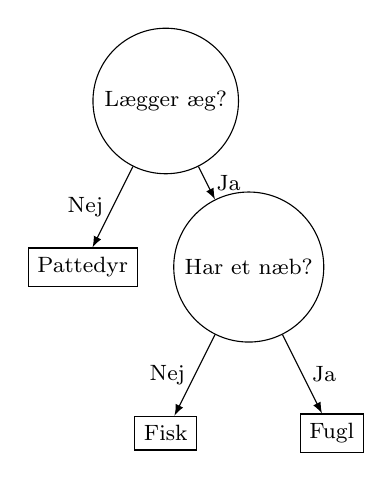
\begin{tikzpicture}
	[
	grow                    = down,
	sibling distance        = 6em,
	level distance          = 6em,
	edge from parent/.style = {draw, -latex},
	every node/.style       = {font=\footnotesize}
	]
	\node [node_] {Lægger æg?}
	child { node [leaf_] {Pattedyr}
		edge from parent node [left] {Nej} }
	child { node [node_] {Har et næb?}
		child { node [leaf_] {Fisk}
			edge from parent node [left]{Nej} }       
		child { node [leaf_] {Fugl}
			edge from parent node [right]{Ja} }
		edge from parent node [right] {Ja} };
	\end{tikzpicture}
\end{center}
Dette ser undertiden fint ud, men prøver man sætte et næbdyr ind i denne model, vil den blive klassificeret som en fugl (da den har et næb og lægger æg), selvom den egentlig er et pattedyr. Selvom vi egentlig har en model, som måske kan klassificere de fleste dyr korrekt, vil der være specielle tilfælde, hvor den skyder helt ved siden af. I dette eksempel kunne man muligvis løse problemet ved at indsamle flere egenskaber, og benytte et større træningssæt, men dette vil ikke altid være muligt, og der vil som sådan være situationer, hvor man ikke kan bygge en perfekt klassificeringsmodel.


\subsection{Beslutningstræer (Decision trees)}
Et eksempel på en klassificeringsteknik er gennem brug af beslutningstræer. Et beslutningstræ består af knuder og blade samt en rodknude. Et datapunkt kan da klassificeres ved at traversere træet startende i roden.

Hver knude består af et spørgsmål, som har en definitiv mængde svar, der kan besvares ud fra egenskaberne i et givent datapunkt. Ud fra svaret (altså datapunktets egenskaber) peger knuden videre til en ny knude eller et blad. Et blad repræsenterer den endelige kategori. I eksemplet i figur 1, kan der ses et eksempel på hvordan et \textit{decision tree} fungere, i dette eksempel antager vi, vi har fået en mængde, som indeholder enten biler, fly eller både, vi starter med at spørge om det givet datapunkt har hjul, hvis nej må det være en båd, hvis ja kan det enten være en bil eller et fly, og derfor spørger vi igen, denne gang om det givet datapunkt har vinger, hvis ja er det et fly, og hvis nej må det være en bil, på denne måde har vi sikret os at vores datapunkt er kommet i den rigtige kategori.

\begin{figure}[H]
\begin{center}
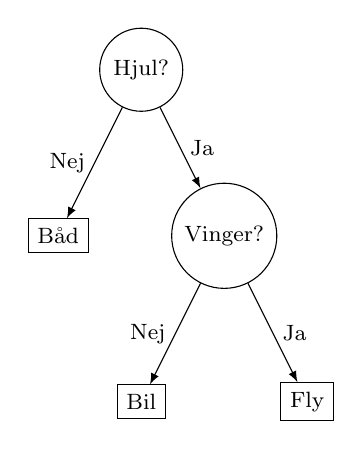
\begin{tikzpicture}
  [
    grow                    = down,
    sibling distance        = 6em,
    level distance          = 6em,
    edge from parent/.style = {draw, -latex},
    every node/.style       = {font=\footnotesize}
  ]
  \node [node_] {Hjul?}
    child { node [leaf_] {Båd}
      edge from parent node [left] {Nej} }
    child { node [node_] {Vinger?}
      child { node [leaf_] {Bil}
              edge from parent node [left]{Nej} }       
      child { node [leaf_] {Fly}
              edge from parent node [right]{Ja} }
              edge from parent node [right] {Ja} };
\end{tikzpicture}
\end{center}
\caption{\textit{Decision tree} eksempel}
\end{figure}

Et (muligvis suboptimalt) beslutningstræ kan bl.a. konstrueres fra et træningssæt med Hunts algoritme. Algoritmen starter med en mængde af alle datapunkter i træningssættet. Hvis alle punkter i mængden har samme kategori bliver denne mængde et blad i træet. Ellers stilles et spørgsmål om punkterne i mængden, og disse punkter uddeles samles i delmængder ud fra, hvordan de besvarer spørgsmålet. Spørgsmålet bliver en knude i træet, som peger på de nye delmængder, og algoritmen køres rekursivt på delmængderne.


\subsubsection{Eksempel på modeludledning}
For at illustrere brugen af decision trees vil vi her vise et eksempel på, hvordan man ud fra et todimensionelt træningssæt og testsæt kan bygge og efterteste en klassificeringsmodel. Betragt følgende træningssæt:

\begin{tabular}{c|c|c}
	X & Y & Klasse\\
	\hline
	0.8 & 0.9 & A\\
	0.6 & 0.1 & B\\
	0.2 & 0.3 & C\\
	0.1 & 0.8 & C\\
	0.4 & 0.2 & B\\
	0.4 & 0.5 & A\\
	0.03 & 0.6 & C\\
	0.5 & 0. 3 & B\\
	0.6 & 0.7 & A\\
	0.45 & 0.8 & A\\
	0.8 & 0.7 & B\\
	0.28 & 0.3 & C\\
	0.1 & 0.05 & C
\end{tabular} 

Tegner vi disse punkter ind i en graf ser det således ud:
\begin{center}
	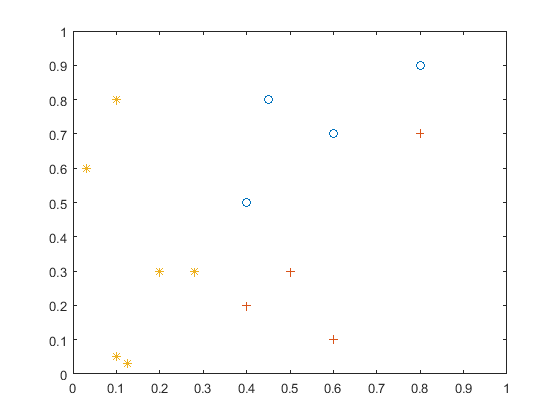
\includegraphics{decision_tree_example_plot}
\end{center}
Hvor blå cirkler er A, røde plusser er B og gule stjerner er C. Der er klare tendenser i, hvordan punkterne har fordelt sig. Ved at indtegne et par linjer kan vi tydeligt illustrere dette:
\begin{center}
	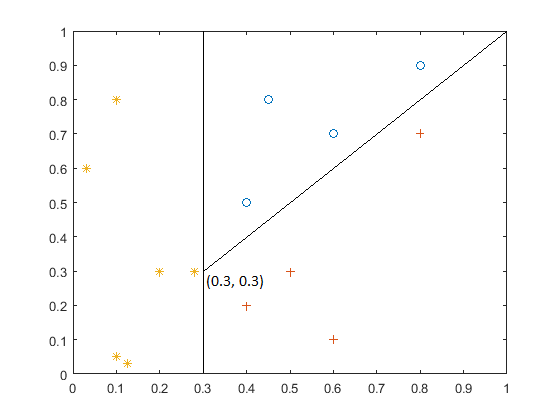
\includegraphics{decision_tree_example_plot_splitted}
\end{center}
Ud fra denne opdeling kunne det tyde på, at $f(x,y)=C$ for $x<0.3$, $f(x,y)=A$ for $0.3<x<y$ og $f(x,y)=B$ for $0.3<x$ og $y<x$. Med disse observationer kan vi bygge et beslutningstræ med Hunts algoritme.

Lad $D_t$ være hele træningssættet. Så indeholder $D_t$ punkter af alle klasser, vælger vi en (\textit{attribute test condition}) ad adskille punkterne på. For at få det mindste træ starter vi med at teste om $x<0.3$, hvilket giver også en mængde $D_{t1}=\{p\ |\ class(p)=C\}$ for ja og $D_{t2}=\{p\ |\ class(p)\neq C\}$ for $0.3<x$. Da $D_{t1}$ kun indeholder en klasse bliver dette til et $C-$blad i træet, mens vi må teste rekursivt på $D_{t2}$.

Vi tester $D_{t2}$ for egenskaben $x<y$ og får en gruppe $D_{t3}=\{p\ | class(p)=A\}$ for ja og $D_{t4}=\{p\ |\ class(p)=B\}$ for nej. Da begge disse grupper er rene (kun indeholder en punkter af en klasse) bliver disse til blade, og vi kan nu tegne vores beslutningstræ.

\begin{center}
	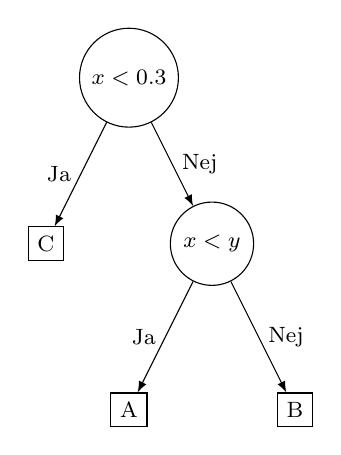
\begin{tikzpicture}
	[
	grow                    = down,
	sibling distance        = 6em,
	level distance          = 6em,
	edge from parent/.style = {draw, -latex},
	every node/.style       = {font=\footnotesize}
	]
	\node [node_] {$x<0.3$}
	child { node [leaf_] {C}
		edge from parent node [left] {Ja} }
	child { node [node_] {$x<y$}
		child { node [leaf_] {A}
			edge from parent node [left]{Ja} }       
		child { node [leaf_] {B}
			edge from parent node [right]{Nej} }
		edge from parent node [right] {Nej} };
	\end{tikzpicture}
\end{center}
Det er nu lykkedes at bygge en model, som kan opdele træningssættet korrekt. Dette er dog ingen garanti for, modellen er korrekt. Modellen er bygget ud fra nogen antagelser, som holder gennem træningssættet, men det betyder ikke, at det holder i praksis. For at undersøge modellens nøjagtighed vil vi bruge den til at klassificere testsættet nedenfor.

\begin{tabular}{c|c|c}
	X & Y & Klasse\\
	\hline
	0.2 & 0.01 & C\\
	0.28 & 0.1 & C\\
	0.1 & 0.2 & C\\
	0.4 & 0.5 & A\\
	0.5 & 0.8 & A\\
	0.9 & 0.95 & A\\
	0.5 & 0.4 & B\\
	0.8 & 0.2 & B\\
	0.6 & 0.5 & A\\
	0.7 & 0.1 & B\\
	0.5 & 0.12 & B\\
	0.12 & 0.75 & C
\end{tabular} 

Tegner vi punkterne ind i en graf med grænserne sat som før får vi følgende resultat:
\begin{center}
	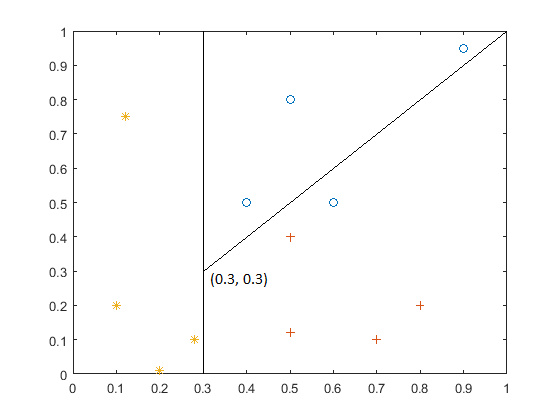
\includegraphics{decision_tree_example_plot_test}
\end{center}
Testsættet passer næsten overens, men der er et enkelt punkt som ikke overholder vores antagelse, så modellen er ikke perfekt. Helt konkret kan vi udregne en nøjagtighed baseret på vores resultat med testsættet. Ud af 12 punkter blev 11 punkter klassificeret korrekt, så vi regner os frem til en nøjagtihed $acc_M=\frac{11}{12}\approx0.92$


\section{Support Vector Machines (SVM)}

En SMV træningsalgoritme er en type klassifikationsteknik til binær klassifikation, som er specielt egnet til data af mange dimensioner. Teknikken baseres på at finde et \textit{maximal margin hyperplane}, altså et hyperplan som deler datapunkterne op i to dele svarende til deres kategori, med maksimal margin til de nærmeste punkter. Dette hyperplan betegnes som modellens \textit{decision boundary}.

Formålet med at maksimere margin er at optimere modellens generaliseringsevne, og dermed opnå bedst mulig nøjagtig når nye punkter skal klassificeres. Hvis vores decision boundary har meget lille margin, er der intuitivt ikke plads til meget forskel på datæn sammenlignet med træningssættet. Dette koncept illustreres i eksemplet nedenfor.

Betragt træningssættet af todimensionelle punkter, markeret som plusser og cirkler afhængig af deres klasse.

\begin{center}
	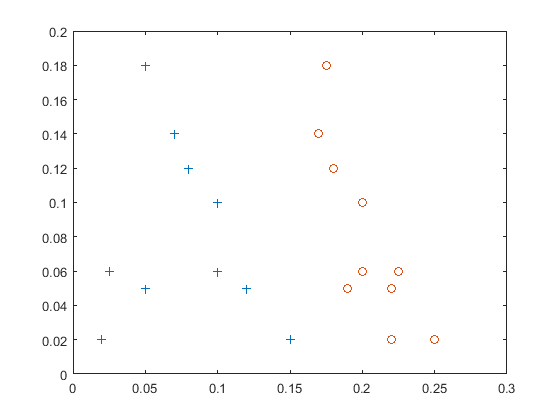
\includegraphics{maximal_margin_hyperplane_1}
\end{center}

Nedenfor er indtegnet to hyperplaner (sorte linjer) og deres margin (grå linjer), som begge deler træningssættet op uden fejl. Det er tydeligt at B2 har breddere margin end B1, og B2 er derfor objektivt den bedste løsning til problemet. Undersøger man selv datæn for en naturlig tendens i opdelingen, bliver det også tydeligt at se, at B2 følger denne tendens langt bedre end B1.

\begin{center}
	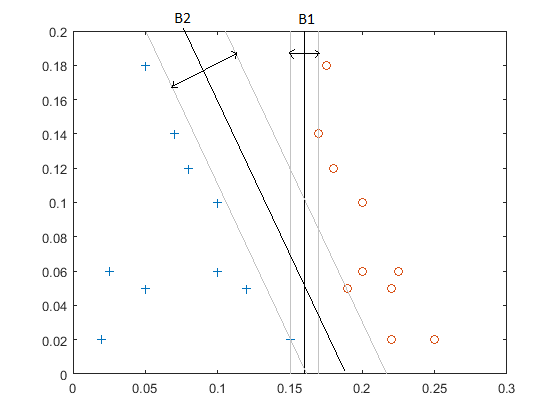
\includegraphics{maximal_margin_hyperplane_2}
\end{center}


\subsection{Linear SVM}
\subsubsection{Separable case}
I vores gennemgang af linear SVM vil vi kigge på et problem hvor vi kan klassificere et dataset i to klasser, vores inddeling kan beskrives mere formelt som $(x_i,y_i) \ i=1,2,...N$ hvor $x_i$ repræsentere det i'te dataset, i disse eksempler vil $y_i \in \{-1,1\}$ dvs. at vi inddeler vores data i to klasser, enten $-1$ eller $1$.

For at finde punkter på vores grænse kan vi opstille ligningen nedenfor, og de punkter der er lig med $0$ vil ligge på grænsen. De to variable $w$ og $b$ er inputs fra modellen, for helt præcist at beskrive dem er $w$ en normal vektor til vores grænse \textit{decision boundary}, og $b$ er den vinkelrette afstand til dens originale punkt.
$$w \cdot x + b = 0$$
På grafen nedenfor kan et eksempel på et plot af dataset set, hvis der lå punkter på $B1$, ville de opfylde betingelserne for ligningen ovenfor.
\begin{center}
	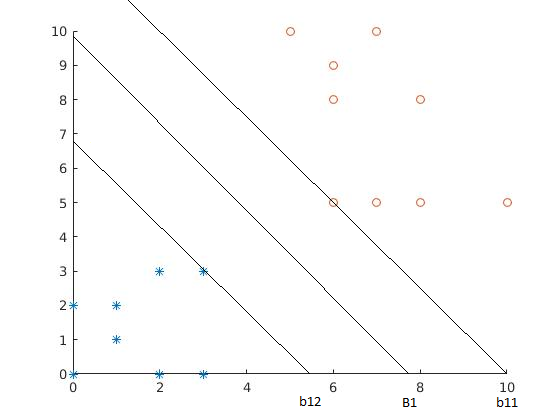
\includegraphics{svm_plot}
\end{center}

For punkter der ligger ved siden af grænsen kan vi opstille en gaffelfunktion, som kan ses nedenfor, de punkter der er mindre end $0$ ligger under grænsen, og vil blive klassificeret som $-1$, og de punkter der er større end $0$ ligger over grænsen og vil blive klassificeret som $1$. Og hvis vi kigger på grafen fra tidligere vil cirklerne blive kvalificeret som $1$, og stjernerne blive kvalificeret som $-1$.
$$
   y_i = \left\{
     \begin{array}{lr}
       1, & if \ w \cdot x_i + b > 0 \\
       -1, & if \ w \cdot x_i + b < 0
     \end{array}
   \right.
$$

Vi kan skalere vores $w$ og $b$1 således at vi finder de punkter der ligger på vores margener. Som det kan ses i den tidligere graf vil det punkt som ligger på $b_{11}$ opfylde den første ligning, og det punkt, som ligger på b12 opfylde den anden ligning. 
$$b_{i1}: w \cdot x + b = 1$$
$$b_{i2}: w \cdot x + b = -1$$

Og da vi gerne vil have de margener med den største afstand fra hinanden kan vi omskrive de forgående ligninger til at kunne beregne afstanden mellem margenerne, dette kan vi gøre ved at indsætte de punkter, som ligger på den ovre og den nedre margen, og ved at trække de to ligninger fra hinanden, kan vi komme frem til den formel, som kan ses nedenfor. Her kan vi se at afstanden mellem de to margener ($d$), kan findes ved $\frac{2}{||w||}$. Og når vi senere hen skal til at optimere $w$, kan det let ses at for at finde den største afstand, skal vi minimere $w$. 
\begin{align*}
w \cdot (x_1 - x_2) = 2 \\
||w|| \times d = 2 \\
d = \frac{2}{||w||} \\
\end{align*}

For at træne vores SVM skal vi estimere $w$ og $b$ således at nedenstående betingelser er overholdt, de skal overholdes på den måde at de dataset som tilhører klassen $1$ skal overholde den første formel, og de dataset som tilhøre klassen $-1$ skal overholde den anden formel. 
$$w \cdot x_i + b \leq 1 \ if \ y_i = 1$$
$$w \cdot x_i + b \geq 1 \ if \ y_i = -1$$

Formlerne ovenfor kan samles til formlen, som kan ses nedenfor, denne formel vil vi bruge i sammenhæng med optimering af $w$ og $b$. 
$$y_i(w \cdot x_i + b) \geq, \ i =1,2,...,N$$

For at opnå den største afstand mellem de to margener, kan vi opstille en objektive funktion, som kan ses nedenfor. Denne objektive funktion skal minimeres.  
$$f(w)=\frac{||w||^2}{2}$$

(Definition)
$$\min\limits_{w} \frac{||w||^2}{2}$$

\subsubsection{Optimering}

For at optimere vores objektive funktion, skal vi bruge \textit{Lagrange multiplier}, \textit{Lagrange multiplier} er en metode der bruges til at finde en funktions minimum eller maksimum, og i dette tilfælde skal vi bruge den til at finde $f(w)=\frac{||w||^2}{2}$ minimum, da dette vil give os den bedste \textit{decision boundary}, vi bruger \textit{Lagranges multiplier} på grund af vores problem består af en objektiv funktion, som er kvadratisk og vores begrænsninger er lineære i parametrene $w$ og $b$, og dette ender ud i at være et konveks optimerings problem, og her bliver \textit{Langranges multiplier} brugt som standard.

For at kunne bruge \textit{Langrange multipliers} bliver vi nød til at omskrive vores objektive funktion, til en ny objektiv funktion, som tager højde for vores begrænsninger, den nye objektive funktion kendes også som en \textit{Langrangian} funktion, variablen $\lambda_i$ i den nye funktion er kendt som en \textit{Langrange multiplier}. 
$$L_P = \frac{1}{2}||w||^2 - \sum\limits_{i=1}^N \lambda_i (y_i(w \cdot x_i + b) - 1)$$
Grunden til at vi har været nødsaget til at ændre vores objektive funktion fra $f(w) = \frac{||w||^2}{2}$ til den overstående objektive funktion er, at den tidligere funktion ville det let ses at for at opnå den minimale værdi ville $w = 0$ være den bedste løsning, men denne løsning ville ikke holde da vores begrænsninger fra $y_i(w \cdot x_i + b) \geq, \ i =1,2,...,N$ ikke ville holde, og hvis vores ulighed ikke holder, vil vi ikke kunne finde en loesning til problemet. Det er her vores \textit{Langrangian} funktion kommer i spil, da den inkorporere vores betingelser i funktionen, og hvis betingelserne ikke holder, vil vaerdien af vores funktion stige, og der ved give et daarlige resultat.

For at kunne minimere vores \textit{Lagrangian} funktion, skal vi først lave to partielle differentieringer, først differentiere vi i forhold til $w$, og derefter differentiere vi i forhold til $b$. Nedenfor kan de to partielle differentieringer ses.
$$\frac{\partial L_p}{\partial w} = 0 \Rightarrow w = \sum\limits_{i=1}^N \lambda_i y_i x_i$$
$$\frac{\partial L_p}{\partial b} = 0 \Rightarrow \sum\limits_{i=1}^N \lambda_i y_i = 0$$
Selvom vi har fundet de partielt differentieret funktioner, er det stadig ikke muligt at finde $w$ og $b$, dette skyldes at vores definition af vores objektive funktion kun indeholder uligheder, og at \textit{Lagrange multiplier} skal bruge ligheder, hvis vores definition havde indeholdt ligheder, ville det havde været muligt at finde værdierne til $w$, $b$ og $\lambda$ med de $N$ ligninger som vi har fundet. Men for at løse dette problem skal vi transformere vores uligheder til ligheder, og dette kan vi gøre med \textit{Karush-Kuhn-Tucker} betingelser, disse betingelser kan ses nedenfor.
$$\lambda_i \geq 0$$
$$\lambda_i[y_i(w \cdot x_i + b) - 1] = 0$$
Som det kan ses i vores nye ligheder, skal alle $\lambda_i$ være $0$ når $y_i(w \cdot x_i + b) \neq 0$, og ud fra dette ved vi at alle de punkter der ligger på $b_{i1}$ eller $b_{i2}$ har en \textit{Lagrange multiplier} $\lambda_i > 0$.  De punkter der ligger paa $b_{i1}$ og $b_{i2}$ og opfylder betingelserne, er ogsaa kendt som \textit{support vectors}.

Vores optimerings problem er stadig kompliceret, grundet vi har $w$, $b$ og $\lambda_i$, vi kan gå hen or simplificere problemet ved at bruge \textit{dual problem} metoden, denne metode bruges ofte i sammenhæng med \textit{Lagrange mlutipliers}, metoden transformere vores \textit{Lagrangian} funktion til en funktion, som kun indeholder vores \textit{Lagrange multipliers}. Nedenfor kan vores \textit{dual problem} funktion ses.
$$L_D = \sum\limits_{i=1}^N \lambda_i - \frac{1}{2}\sum\limits_{i,j} \lambda_i \lambda_j y_i y_j x_j \cdot x_j$$
Der er to store forskelle på vores primære \textit{Lagrangian} funktion, og vores nye \textit{dual problem} funktion. Den første store forskel er at vores \textit{dual problem} kun indeholder vores trænings data samt vores \textit{Lagrange multipliers}, hvor at i vores primære \textit{Lagrangian} funktion også indeholder vores $w$ og $b$. Den anden store forskel er at vores minimerings problem  er blevet til et maksimerings problem.
Løsningen af vores \textit{dual problem} vil vi ikke bruge mere tid på, dette skyldes at bogen nævner at det kan løses med \textit{quadritic programming}, men at det er udover bogens indhold. \\
(TODO COMPLETE)
$$( \sum\limits_{i=1}^N \lambda_i y_i x_i \cdot x) + b = 0$$

Når vi endelig er færdig med at beregne alle vores parametre for vores grænse, kan vi stille en funktionen op, som kan ses nedenunder, den funktion kan beregne hvilke klassifisering det givet dataset $z$ tilhøre, hivs $f(z) = 1$ vil $z$ blive klassificeret som $1$ ellers vil $z$ blive kvalificeret som $-1$. 
$$f(z) = sign(w \cdot z + b) = sign( \sum\limits_{i=1}^N \lambda_i y_i x_i \cdot z + b)$$

\subsubsection{Non-separable case}
I nogle tilfælde vil den bedste grænse (\textit{dicision boundary}) ikke altid opdele alle vores dataset, men der vil være enkelte dataset, som bliver klassificeret forkert, dette kan skyldes forskellige ting såsom fejl i trænings data, eller at der er et enkelt dataset, som ikke holder sig til mønstret for dens klassificering. Men i disse tilfælde vil vi stadig prøve at opnå så stor en afstand mellem vores magner som muligt, selvom enkelte dataset bliver klassificeret forkert, dette skyldes at hvis vi valgte en grænse, som ville opdele vores dataset uden fejl, ofte ville have en meget lille afstand mellems dens magner, og dette vil gøre at modellen ville være meget udsat for \textit{overfitting}. På grafen nedenfor ses et eksempel hvor at $B2$ ville være den oplagte grænse at vælge, da den opdeler alt data korrekt, men vi også vælge $B1$ grundet at den har en større afstand mellem sine margener, og chancen for \textit{overfitting} ville være mindre. 
\begin{center}
	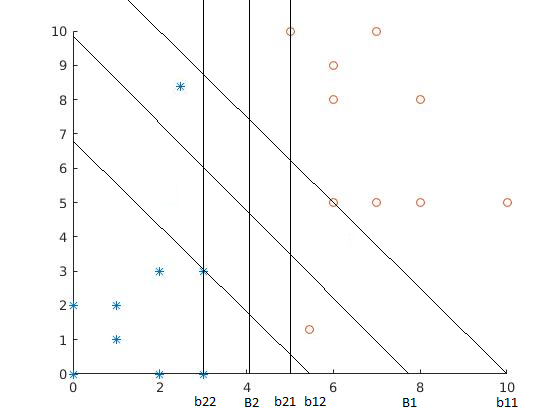
\includegraphics{svm_plot_1}
\end{center}
Grundet at vi har punkter der ikke er klassificeret rigtigt af vores grænsen, vil vores tidligere ligninger ikke passer på alle vores dataset, og for at rette dette introducere vi \textit{slack variables} ($\xi$), disse variabler skal placere de dataset der er kvalificeret forkert rigtigt, og dette gøres ved at addere eller substakterre (hvilke der skal bruges kommer an på hvor datasettet er placeret) med vores nye variable ($\xi$). 

 Som det kan ses i vores to nye ligninger skal vi subtrakterer hvis vores dataset er placeret under grænsen, men den skal kvalificeres, som om den lå oven for grænsen, dette gør vi ved at subtrakterer højre siden af ligningen med vores \textit{slack variable}, med en værdi som gør at formlen er sand. Det samme gælder for det omvendte scenarie, men her bruges addition på højre siden af ligningen for at få ligningen til at blive sand.  
$$w * x_i + b \geq 1 - \xi_i \ if \ y_i = 1$$
$$w * x_i + b \leq 1 - \xi_i \ if \ y_i = -1$$
Bemærk $\forall i : \xi_i > 0$

Men for ikke bare at vælge en grænse med store magner, og så bare rette alle de forkerte klassificeret dataset til med \textit{slack variables}, introducere vi en vægt for hvert dataset, som er kvalificeret forkert, denne vægt kan ses i den modificeret objektive funktion nedenfor, bemærk at $C$ og $k$ bliver sat a brugeren (ofte vil $k = 1$ grundet simplicitet). Det ses klart at for hvert punkt, som er kvalificeret forkert vil de valgte margener blive rangeret dårligere. 

$$f(w) = \frac{||w||^2}{2}+C(\sum\limits_{i=1}^N \xi_i)^k$$

\subsubsection{Optimering}
Optimering med vores \textit{slack variable} er næsten ens med vores optimering uden vores ekstra variable. Igen vil vi starte med at lave vores objektive funktion om til en \textit{Lagrangian} funktion.
$$L_P = \frac{1}{2}||w||^2 + C \sum\limits_{i=1}^N \xi_i - \sum\limits_{i=1}^N \lambda_i (y_i(w \cdot x_i + b) - 1 + \xi_i) - \sum\limits_{i=1}^N \mu_i \xi_i$$
For at forstå funktionen er det nemmest hvis man deler den op, funktionen kan deles op i fire dele, hvor de to første dele er vores objektive funktion, som vi prøver at minimere, de tredje del  er repræsentere vores uligheder, 

\subsection{Non-linear SVM}
Det er ikke altid muligt at definere en lineær opdeling af datæn. En naiv løsning på dette problem er, at transformere datapunkterne til et andet rum, hvor en lineær opdeling er mulig.

Antag at vi har en transformation $\Phi(x)$ fra det originale rum til et transformeret rum, hvor en lineær opdeling er mulig. Så kan vi genbruge vores viden fra det lineære tilfælde, og optimeringen er nogenlunde den samme. For at opnå den maksimale margin skal vi igen minimere funktionen 
$$f(w)=\frac{||w||^2}{2}$$
Under kravet at
$$y_i(w\cdot\Phi(x_i)+b)\geq 1,\text{ for }i=1,2..,N$$
Ligningen er næsten identisk med det lineære tilfælde, men vi optimerer nu med $\Phi(x_i)$ - altså $x_i$ i det transformerede rum.

Lagrange kan nu benyttes på samme måde som i det lineære tilfælde. Også her skal vi blot benytte de transfomerede punkter.

\begin{align*}
L_D&=\sum_{i=1}^{n}\lambda_i-\frac{1}{2}\sum_{i,j}\lambda_i\lambda_j y_iy_j\Phi(x_i)\cdot\Phi(x_j)
\end{align*}

Denne optimering kræver som man kan se udregningen af prikproduktet mellem samtlige par af punkter i det transformerede rum. Da dette kan være udregningsmæssigt tungt, og kræver at man kender en transformation der passer på det enkelte problem, vil man typisk bruge en anden tilgang kaldet \textit{kernel trick}, som tillader os at benytte kernefunktioner til at opnå et ækvivalent resultat.


\subsubsection{Kernefunktioner}
Lad $X=\{x_1..x_n\}\subset \chi_1$ være en mængde af $n$ vektorer i rummet $\chi_1$, og lad $\Phi:\chi_1\rightarrow\chi_2$. Da er en kernefunktion $k$ med feature mapping $\Phi$ en funktion der udregner det indre produkt af ethvert vektorpar $x_i,x_j\in X$ transformeret til $\chi_2$. Altså
\begin{equation}
k(x_i,x_j)=\langle\Phi(x_i),\Phi(x_j)\rangle
\end{equation}

Så definerer vi kernen $K$ som en $n\times n$-matrice med indre produkter af input vektorerne
\begin{equation}
K=\left[\begin{array}{r r r}
\langle\Phi(x_1),\Phi(x_1)\rangle & ... & \langle\Phi(x_1),\Phi(x_n)\rangle\\
 & ... & \\
\langle\Phi(x_n),\Phi(x_1)\rangle & ... & \langle\Phi(x_n),\Phi(x_n)\rangle\\
\end{array}\right]\\
\end{equation}
Et indre produkt er per definition symmetrisk, så det følger at
\begin{equation}
K_{i,j}=\langle\Phi(x_i),\Phi(x_j)\rangle=\langle\Phi(x_j),\Phi(x_i)\rangle=K_{j,i}
\end{equation}
Hvilket viser at $K$ må være symmetrisk over diagonalen. 

Foruden den symmetriske egenskab skal $K$ være positiv semidefinit for at $k$ er en gyldig kernefunktion. $K$ betegnes da som Gram matricen for det indre produkt i $\chi_1$. Dette betyder formelt at
\begin{equation}
\forall c\in R^n,c^TKc\geq 0
\end{equation}




Med denne definition kan $k$ nu erstatte prikproduktet og transformationerne i Lagrange problemet:
\begin{align*}
L_D&=\sum_{i=1}^{n}\lambda_i-\frac{1}{2}\sum_{i,j}\lambda_i\lambda_j y_iy_jK(x_i,x_j)
\end{align*}


\end{document}